\chapter{Graphs}
\section{The Basics}

% 1.1 Recall (Text Block)
\topic{Recall}

\begin{enumerate}
    \item A \textbf{set} is merely an accumulation of objects. These objects are called \textbf{elements} of the set. If an object $x$ is an element of $S$, we write $x \in S$. The set of all elements with a certain property $P$ is denoted via $\{x \mid x \text{ has property } P\}$.
    
    \item An \textbf{$n$-ary relation} $R$ on a set $A$ is a subset of the power set of $A^n$, i.e., $R \subseteq \mathcal{P}(A^n)$. If $n=2$, we call the relation \textbf{binary}.
    
    A binary relation $R$ on a set $A$ is called:
    \begin{itemize}
        \item[(i)] \textbf{symmetric} if $R(a,b)$ implies $R(b,a)$ for all $a,b \in A$.
        \item[(ii)] \textbf{asymmetric} if $R(a,b)$ implies $\neg R(b,a)$ for all $a,b \in A$.
        \item[(iii)] \textbf{antisymmetric} if $R(a,b) \land R(b,a)$ implies $a=b$ for all $a,b \in A$.
        \item[(iv)] \textbf{reflexive} if $R(a,a)$ for all $a \in A$.
        \item[(v)] \textbf{irreflexive} if $\neg R(a,a)$ for all $a \in A$.
        \item[(vi)] \textbf{transitive} if $R(a,b) \land R(b,c)$ implies $R(a,c)$ for all $a,b,c \in A$.
    \end{itemize}
\end{enumerate}

% 1.2 Definition (Red Box)
\begin{definition}
A \textbf{graph} $G=(V,E)$ is a pair of sets $V$ and $E$ such that $E$ consists of subsets of $V$ of size two. $V$ is called the set of \textbf{vertices} and $E$ the set of \textbf{edges}. A graph $G$ is called \textbf{finite} if $V$ is a finite set. The \textbf{order} $|G|$ of a graph $G=(V,E)$ is the cardinality of its vertex set, so $|G|=|V|$. The \textbf{size} $\|G\|$ of $G$ is the cardinality of its edge set, $\|G\|=|E|$.
\end{definition}

% 1.3 Visualisation (Text Block)
\topic{Visualisation}

Let $G=(V,E)$ be a graph. We visualise vertices $u,v \dots \in V$ by dots and edges $e=\{u,v\} \in E$ by the diagram:

\begin{center}
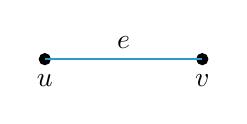
\begin{tikzpicture}
    \filldraw (0,0) circle (2pt) node[below=2pt] {$u$};
    \filldraw (2,0) circle (2pt) node[below=2pt] {$v$};
    \draw[cyan!80!black, thick] (0,0) -- (2,0) node[midway, above, black] {$e$};
\end{tikzpicture}
\end{center}

% 1.4 Example (Text Block)
\begin{example}[Bowtie Graph]
Let $G=(V,E)$ be the graph with $V=\{a,b,c,d,e\}$ and
\[ E = \{\{a,b\}, \{a,c\}, \{a,d\}, \{a,e\}, \{b,c\}, \{d,e\}\}. \]
The graph $G$ has order 5 and size 6. It can be visualized via:
\begin{center}
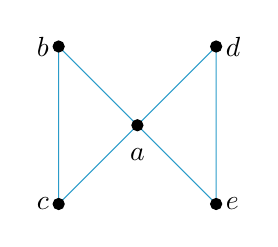
\begin{tikzpicture}
    \coordinate (a) at (0,0);
    \coordinate (b) at (-1,1);
    \coordinate (c) at (-1,-1);
    \coordinate (d) at (1,1);
    \coordinate (e) at (1,-1);

    \draw[cyan!80!black] (b) -- (a) -- (c) -- (b);
    \draw[cyan!80!black] (d) -- (a) -- (e) -- (d);

    \filldraw (a) circle (2pt) node[below=5pt] {$a$};
    \filldraw (b) circle (2pt) node[left] {$b$};
    \filldraw (c) circle (2pt) node[left] {$c$};
    \filldraw (d) circle (2pt) node[right] {$d$};
    \filldraw (e) circle (2pt) node[right] {$e$};
\end{tikzpicture}
\end{center}
This visualisation motivates its name: \textbf{bowtie graph}.
\end{example}

% 1.5 Notation
\topic{Notation}

\begin{enumerate}
    \item For a graph $G=(V,E)$ we may denote its vertex set by $V(G)$ or $V_G$ for clarity.
    \item Similarly, we often denote $E$ by $E(G)$ or $E_G$.
    \item We denote an edge $\{u,v\}$ simply by $uv$.
    \item Edges are often called $e, e_1, e_2, f \dots$, while vertices are called $u, v, x, y, \dots$.
\end{enumerate}

% 1.6 Definition
\begin{definition}
Let $G=(V,E)$ be a graph.
\begin{enumerate}
    \item If $uv \in E$ is an edge, then we say that $u$ and $v$ are \textbf{adjacent} or \textbf{neighbours}. If $uv \notin E$, we call $u$ and $v$ \textbf{nonadjacent}.
    \item If $e=uv \in E$, we say that $u$ and $v$ are the \textbf{end vertices} of $e$ or that they are \textbf{incident} with $e$.
    \item The \textbf{neighborhood} $N(v)$ of a vertex $v \in V$ is the set of all vertices adjacent to $v$, i.e., $N(v) = \{u \in V \mid uv \in E\}$. The \textbf{closed neighborhood} $N[v]$ of $v$ is $N[v] := N(v) \cup \{v\}$.
    \item The \textbf{neighborhood} $N(S)$ of a set of vertices is defined as $N(S) := \bigcup_{v \in S} N(v)$. Similarly, the \textbf{closed neighborhood} $N[S]$ is set to be $N[S] := N(S) \cup S (= \bigcup_{v \in S} N[v])$.
    \item The \textbf{degree} $\deg(v)$ of $v \in V$ is the number of edges incident with $v$, i.e., $\deg(v) := |\{e \in E \mid v \in e\}| = |N(v)|$.
    \item The \textbf{maximum degree} $\Delta(G)$ of $G$ is defined as
    \[ \Delta(G) := \max \{ \deg(v) \mid v \in V \}. \]
    Similarly, $\delta(G) := \min \{ \deg(v) \mid v \in V \}$ is the \textbf{minimum degree} of $G$.
    \item The \textbf{degree sequence} of a graph $G$ is the sequence containing all degrees of the vertices of $G$ (with repetition) in decreasing order.
\end{enumerate}
\end{definition}

% 1.7 Example
\begin{example}
Consider $G$ given by:
\begin{center}
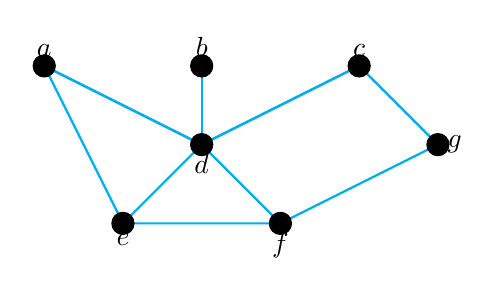
\begin{tikzpicture}[scale=2]
    \coordinate (a) at (0,1);
    \coordinate (b) at (1,1);
    \coordinate (c) at (2,1);
    \coordinate (d) at (1,0.5);
    \coordinate (e) at (0.5,0);
    \coordinate (f) at (1.5,0);
    \coordinate (g) at (2.5,0.5);

    % Edges (Cyan color to match notes)
    \draw[cyan, thick] (a) -- (d) -- (c) -- (g) -- (f) -- (e) -- (a); % Outer cycle
    \draw[cyan, thick] (a) -- (d);
    \draw[cyan, thick] (b) -- (d);
    \draw[cyan, thick] (c) -- (d);
    \draw[cyan, thick] (e) -- (d);
    \draw[cyan, thick] (f) -- (d);

    \foreach \point in {a,b,c,d,e,f,g} \filldraw (\point) circle (2pt);
    \node[above] at (a) {$a$}; \node[above] at (b) {$b$}; \node[above] at (c) {$c$};
    \node[below] at (d) {$d$}; \node[below] at (e) {$e$}; \node[below] at (f) {$f$}; \node[right] at (g) {$g$};
\end{tikzpicture}
\end{center}
Then $\Delta(G)=5$, $\delta(G)=1$. $N(e)=\{a,d,f\}$, $N[b]=\{b,d\}$. $N[a,g]=\{a,c,d,e,f,g\}$
Order of $G$, size of $G$ is 9. Degree sequence $(5,3,3,2,2,2,1)$.
\end{example}

% 1.8 Example
\begin{example}
Consider $G$ given via the diagram:
\begin{center}
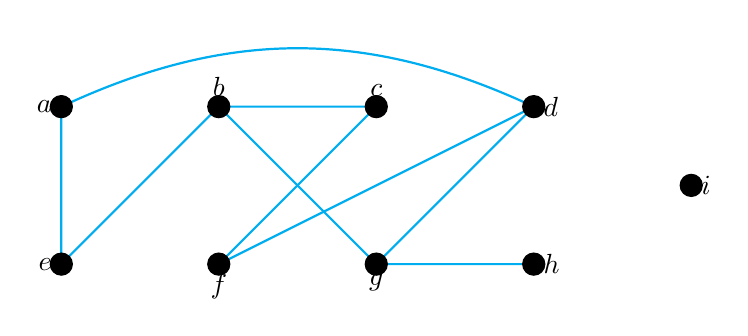
\begin{tikzpicture}[scale=2]
    \coordinate (a) at (0,1); \node[left] at (a) {$a$};
    \coordinate (b) at (1,1); \node[above] at (b) {$b$};
    \coordinate (c) at (2,1); \node[above] at (c) {$c$};
    \coordinate (d) at (3,1); \node[right] at (d) {$d$};
    
    \coordinate (e) at (0,0); \node[left] at (e) {$e$};
    \coordinate (f) at (1,0); \node[below] at (f) {$f$};
    \coordinate (g) at (2,0); \node[below] at (g) {$g$};
    \coordinate (h) at (3,0); \node[right] at (h) {$h$};
    \coordinate (i) at (4,0.5); \node[right] at (i) {$i$};
    
    % Edges (Cyan color to match notes)
    \draw[cyan, thick] (h) -- (g) -- (d) -- (f) -- (c) -- (b) -- (e) -- (a); % Outer cycle
    \draw[cyan, thick] (b) -- (g);
    \draw[cyan, thick] (a) to[bend left=25] (d); % {a,d} curved top
    
    \foreach \p in {a,b,c,d,e,f,g,h,i} \filldraw (\p) circle (2pt);
\end{tikzpicture}
\end{center}

Then $V(G)=\{a,b,c,d,e,f,g,h,i\}$ \\
$E(G)=\{\{a,d\}, \{a,e\}, \{b,c\}, \{b,e\}, \{b,g\}, \{c,f\}, \{d,f\}, \{d,g\}, \{g,h\}\}$

Order $|G|=9$, size of $G$ is 9, degree sequence $(3,3,3,2,2,2,2,1,0)$. \\
$N(f)=\{c,d\}$, $N[d,e]=\{a,b,c,d,e,f\}$, $\Delta(G)=3$, $\delta(G)=0$. 
\end{example}

% 1.9 Remark
\begin{remark}
A graph can be considered as a set $V$ together with a binary relation $E$ on $V$ which is symmetric and irreflexive.
\end{remark}

% 1.10 Definition
\begin{definition}[Variants of Graphs]
\begin{enumerate}
    \item If $G=(V,E)$ and we replace $E$ with a set of ordered pairs, then we call $G$ a \textbf{\color{red}directed graph} or \textbf{\color{red}digraph}.
    \\[0.2cm]
    \textbf{Ex:} $V(G)=\{a,b,c,d\}$, $E(G)=\{(a,b), (a,c), (a,d), (d,a), (d,c)\}$
    \begin{center}
    \begin{tikzpicture}[scale=1.2]
        \coordinate (a) at (0,0);
        \coordinate (b) at (1,1.5);
        \coordinate (c) at (1,-0.5);
        \coordinate (d) at (2,0.5);

        % Edges with LARGE arrows
        % {Stealth[scale=1.5]} makes the arrowhead 50% bigger
        \tikzset{arrowstyle/.style={-{Stealth[scale=1]}, very thick, cyan!80!black}}

        \draw[arrowstyle] (a) -- (b);
        \draw[arrowstyle] (a) -- (c);
        \draw[arrowstyle] (d) -- (c);
        
        % Curved edges for a <-> d
        \draw[arrowstyle] (a) to[bend left=15] (d);
        \draw[arrowstyle] (d) to[bend left=15] (a);

        % Nodes
        \foreach \p/\pos/\label in {a/below left/a, b/above/b, c/below/c, d/right/d}
            \filldraw (\p) circle (2pt) node[\pos] {$\label$};
    \end{tikzpicture}
    \end{center}

    \item If $G=(V,E)$ and we replace $E$ by a multiset (iterations of the same elements are distinguished), then we call $G$ a \textbf{\color{red}multigraph}.
    \\[0.2cm]
    \textbf{Ex:} $E = [\{a,c\}, \{b,c\}, \{b,c\}, \{b,c\}]$
    \begin{center}
    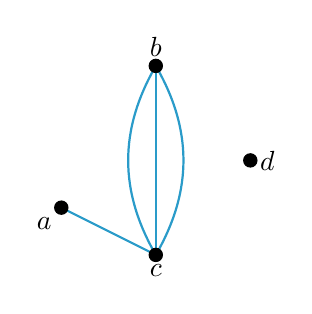
\begin{tikzpicture}[scale=1.2]
        \coordinate (a) at (0,0);
        \coordinate (b) at (1,1.5);
        \coordinate (c) at (1,-0.5);
        \coordinate (d) at (2,0.5); % Isolated node d in drawing

        % Edges
        \draw[thick, cyan!80!black] (a) -- (c);
        \draw[thick, cyan!80!black] (b) -- (c); % Middle edge
        \draw[thick, cyan!80!black] (b) to[bend right=30] (c);
        \draw[thick, cyan!80!black] (b) to[bend left=30] (c);

        % Nodes
        \foreach \p/\pos/\label in {a/below left/a, b/above/b, c/below/c, d/right/d}
            \filldraw (\p) circle (2pt) node[\pos] {$\label$};
    \end{tikzpicture}
    \end{center}

    \item If $G=(V,E)$ and we extend $E$ by allowing loops, we call $G$ a \textbf{\color{red}pseudograph}.
    \\[0.2cm]
    \textbf{Ex:} $E=\{\{a,b\}, \{b,d\}, \{c,c\}, \{d,d\}\}$
    \begin{center}
    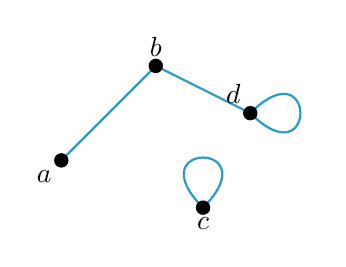
\begin{tikzpicture}[scale=1.2]
        \coordinate (a) at (0,0);
        \coordinate (b) at (1,1);
        \coordinate (c) at (1.5,-0.5);
        \coordinate (d) at (2,0.5);

        % Edges
        \draw[thick, cyan!80!black] (a) -- (b);
        \draw[thick, cyan!80!black] (b) -- (d);
        
        % Loops
        \draw[thick, cyan!80!black] (d) to[out=-45,in=45,loop, min distance=10mm] (d);
        \draw[thick, cyan!80!black] (c) to[out=45,in=135,loop, min distance=10mm] (c);

        % Nodes
        \foreach \p/\pos/\label in {a/below left/a, b/above/b, c/below/c, d/above left/d}
            \filldraw (\p) circle (2pt) node[\pos] {$\label$};
    \end{tikzpicture}
    \end{center}

    \item If we allow edges to be arbitrary sets of vertices instead of 2-elementary ones, we call $G$ a \textbf{\color{red}hypergraph}.
    \\[0.2cm]
    \textbf{Ex:} $E=\{\{a\}, \{a,b,d\}, \{b,c,d\}, \{c,d\}\}$
    \begin{center}
    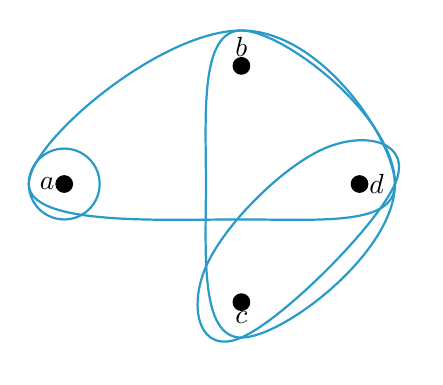
\begin{tikzpicture}[scale=1.5]
        \coordinate (a) at (0,0.5);
        \coordinate (b) at (1.5,1.5);
        \coordinate (c) at (1.5,-0.5);
        \coordinate (d) at (2.5,0.5);

        % Hyperedges (Blobs)
        % {a}
        \draw[thick, cyan!80!black] (a) circle (0.3cm);
        
        % {c,d}
        \draw[thick, cyan!80!black] plot [smooth cycle, tension=0.8] coordinates { (1.5,-0.8) (2.8,0.5) (2.2,0.8) (1.2,-0.2) };
        
        % {a,b,d} - Large curvy shape
        \draw[thick, cyan!80!black] plot [smooth cycle, tension=0.8] coordinates { (-0.3,0.5) (1.5,1.8) (2.8,0.5) (1.5,0.2) };
        
        % {b,c,d} - Vertical curvy shape
        \draw[thick, cyan!80!black] plot [smooth cycle, tension=0.8] coordinates { (1.5,1.8) (2.8,0.5) (1.5,-0.8) (1.2,0.5) };

        % Nodes
        \foreach \p/\pos/\label in {a/left/a, b/above/b, c/below/c, d/right/d}
            \filldraw (\p) circle (2pt) node[\pos] {$\label$};
    \end{tikzpicture}
    \end{center}
\end{enumerate}
\end{definition}

% 1.11 Setting
\topic{Setting}
In this lecture, unless otherwise stated, by a graph we mean a finite, simple graph with $|V| \ge 1$.

% 1.12 Definition
\begin{definition}
\begin{itemize}
    \item The \textbf{\color{red}complete graph $K_n$} for $n \ge 1$ is the graph consisting of $n$ vertices such that any two vertices are adjacent.
    \\[0.2cm]
    \textbf{e.g.}
    \begin{center}
    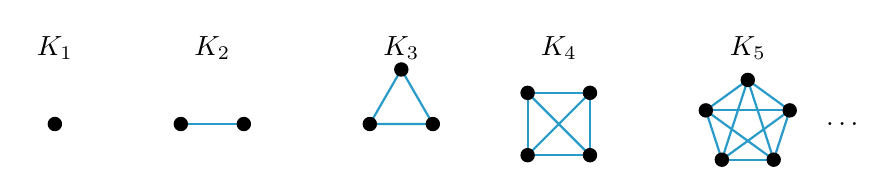
\begin{tikzpicture}[scale=0.8]
        % K1
        \node at (0, 1.2) {$K_1$};
        \filldraw (0,0) circle (3pt);

        % K2
        \begin{scope}[xshift=2cm]
            \node at (0.5, 1.2) {$K_2$};
            \draw[cyan!80!black, thick] (0,0) -- (1,0);
            \filldraw (0,0) circle (3pt);
            \filldraw (1,0) circle (3pt);
        \end{scope}

        % K3
        \begin{scope}[xshift=5cm]
            \node at (0.5, 1.2) {$K_3$};
            \coordinate (a) at (0,0); 
            \coordinate (b) at (1,0); 
            \coordinate (c) at (0.5, 0.866);
            \draw[cyan!80!black, thick] (a)--(b)--(c)--(a);
            \foreach \p in {a,b,c} \filldraw (\p) circle (3pt);
        \end{scope}

        % K4
        \begin{scope}[xshift=8cm]
            \node at (0, 1.2) {$K_4$};
            \foreach \i in {1,...,4} \coordinate (v\i) at (90*\i+45:0.7); 
            \foreach \i in {1,...,4}
                \foreach \j in {\i,...,4}
                    \draw[cyan!80!black, thick] (v\i) -- (v\j);
            \foreach \i in {1,...,4} \filldraw (v\i) circle (3pt);
        \end{scope}

        % K5
        \begin{scope}[xshift=11cm]
            \node at (0, 1.2) {$K_5$};
            \foreach \i in {1,...,5} \coordinate (v\i) at (90+72*\i:0.7);
            \foreach \i in {1,...,5}
                \foreach \j in {\i,...,5}
                    \draw[cyan!80!black, thick] (v\i) -- (v\j);
            \foreach \i in {1,...,5} \filldraw (v\i) circle (3pt);
            
            \node at (1.5,0) {$\dots$};
        \end{scope}
    \end{tikzpicture}
    \end{center}

    \item The \textbf{\color{red}empty graph $E_n$} is the graph consisting of $n$ vertices and no edges.
    \\[0.2cm]
    \textbf{e.g.}
    \begin{center}
    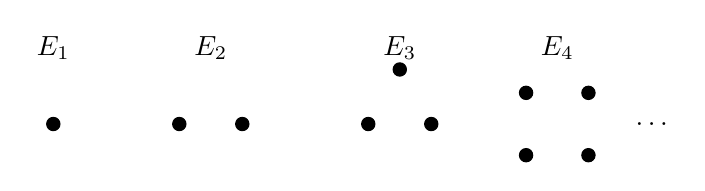
\begin{tikzpicture}[scale=0.8]
        % E1
        \node at (0, 1.2) {$E_1$};
        \filldraw (0,0) circle (3pt);

        % E2
        \begin{scope}[xshift=2cm]
            \node at (0.5, 1.2) {$E_2$};
            \filldraw (0,0) circle (3pt);
            \filldraw (1,0) circle (3pt);
        \end{scope}

        % E3
        \begin{scope}[xshift=5cm]
            \node at (0.5, 1.2) {$E_3$};
            \coordinate (a) at (0,0); 
            \coordinate (b) at (1,0); 
            \coordinate (c) at (0.5, 0.866);
            \foreach \p in {a,b,c} \filldraw (\p) circle (3pt);
        \end{scope}

        % E4
        \begin{scope}[xshift=8cm]
            \node at (0, 1.2) {$E_4$};
            \foreach \i in {1,...,4} \coordinate (v\i) at (90*\i+45:0.7); 
            \foreach \i in {1,...,4} \filldraw (v\i) circle (3pt);
            
            \node at (1.5,0) {$\dots$};
        \end{scope}
    \end{tikzpicture}
    \end{center}
\end{itemize}
\end{definition}

% 1.13 The Handshaking Lemma
% 1.13 The Handshaking Lemma
\begin{theorem}[The Handshaking Lemma]
If $G=(V,E)$ is a graph, then
\[ \sum_{v \in V} \deg(v) = 2|E|. \quad (*) \]
\end{theorem}

\begin{proof}
We proceed by induction on $n := |E|$.

\vspace{0.3cm}
\noindent \underline{\textbf{n=0:}} If $|E|=0$, then $\deg(v)=0$ for any $v \in V$, whence clearly
\[ 0 = \sum_{v \in V} \deg(v) = 2|E| = 0. \]

\vspace{0.3cm}
\noindent \underline{\textbf{n $\to$ n+1:}} Assume $(*)$ holds for any $G'=(V',E')$ with $|E'|=n$ (I.H.) and consider $G=(V,E)$ with $|E|=n+1 (\ge 1)$ arbitrary. Let $e \in E$ arbitrary and consider $G'=(V, E \setminus \{e\})$. Then, if $e=uv$, we get $|E(G)| = |E(G')|+1$ and
\[ \deg_G(u) = \deg_{G'}(u) + 1 \quad \text{and} \quad \deg_G(v) = \deg_{G'}(v) + 1, \text{ whence} \]

\vspace{-0.2cm}
\begin{align*}
    2|E(G)| &= 2|E(G')| + 2 \\
    &\overset{\text{I.H.}}{=} \sum_{w \in V} \deg_{G'}(w) + 2 \\
    &= \sum_{w \in V \setminus \{u,v\}} \deg_{G'}(w) + \deg_{G'}(u) + 1 + \deg_{G'}(v) + 1 \\
    &= \sum_{w \in V} \deg_G(w), \quad \text{as desired.} \qedhere
\end{align*}
\end{proof}

% 1.14 Corollary
\begin{corollary}
Any graph $G$ has an even number of vertices of odd degree.
\end{corollary}
\begin{proof}
Exercise.
\end{proof}

% 1.15 Corollary
\begin{corollary}
For any graph $G=(V,E)$ we have
\[ \delta(G) \le 2 \frac{|E|}{|V|} \le \Delta(G). \]
\end{corollary}
\begin{proof}
\[ |V| \cdot \delta(G) = \sum_{v \in V} \delta(G) \le \sum_{v \in V} \deg(v) \le \sum_{v \in V} \Delta(G) = |V|\Delta(G) \]
Using Theorem 1.13, $\sum \deg(v) = 2|E|$. Dividing by $|V|$ yields the result.
\end{proof}

% 1.16 Lemma
\begin{lemma}
If $|G| \ge 2$, then $G$ contains at least two vertices of the same degree.
\end{lemma}
\begin{proof}
If $G$ has two vertices of degree 0, then we are done. Otherwise, we may assume that $G$ has none. If $|G|=n$, and $v \in V$, then $1 \le \deg(v) \le n-1$. Note that this leaves us with $n-1$ choices of degrees for $n$ many different vertices. Hence, at least two vertices must have the same degree.
\end{proof}

% 1.17 Remark
\begin{remark}
The above line of thought is called the \textbf{pigeon hole principle}. If there are $n$ many pigeons wanting to fit into $n-1$ many holes, then at least two of them have to cuddle up in the same hole.
\end{remark}

% 1.18 Definition
\begin{definition}
\begin{enumerate}
    \item[1)] The \textbf{\color{red}path $P_n$} is the graph on $n$ vertices $v_1, \dots, v_n$ with the edge set $E(P_n) = \{v_i v_{i+1} \mid 1 \le i < n\}$, i.e. $P_n$ is represented by the diagram
    \begin{center}
    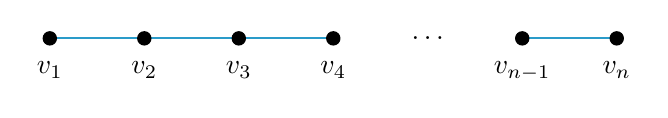
\begin{tikzpicture}[scale=1.2]
        \draw[cyan!80!black, thick] (0,0) -- (3,0);
        \foreach \x/\l in {0/v_1, 1/v_2, 2/v_3, 3/v_4}
            \filldraw (\x,0) circle (2pt) node[below=5pt] {$\l$};
        
        \node at (4,0) {$\dots$};
        
        \draw[cyan!80!black, thick] (5,0) -- (6,0);
        \filldraw (5,0) circle (2pt) node[below=5pt] {$v_{n-1}$};
        \filldraw (6,0) circle (2pt) node[below=5pt] {$v_n$};
    \end{tikzpicture}
    \end{center}

    \item[2)] The \textbf{\color{red}cycle $C_n$} is the graph on $n$ vertices with edge set $E(C_n) = \{v_i v_{i+1} \mid 1 \le i < n\} \cup \{v_n v_1\}$. E.g.
    \begin{center}
    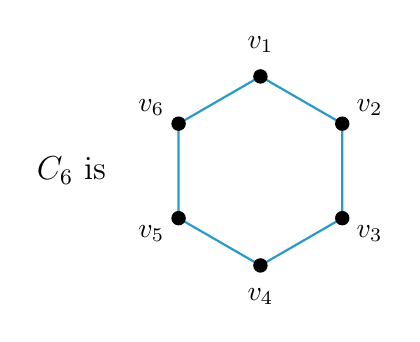
\begin{tikzpicture}[scale=1.2]
        \node at (-2, 0) {\large $C_6$ is};
        
        % Define coordinates first
        \foreach \i in {1,...,6} {
            % Angle: Start at 90 (v1), rotate clockwise by 60 degrees
            \pgfmathsetmacro{\ang}{90 - (\i-1)*60}
            \coordinate (v\i) at (\ang:1);
        }
        
        % Draw edges
        \draw[cyan!80!black, thick] (v1)--(v2)--(v3)--(v4)--(v5)--(v6)--(v1);
        
        % Draw nodes and labels
        \foreach \i in {1,...,6} {
            \pgfmathsetmacro{\ang}{90 - (\i-1)*60}
            % shift={(\ang:0.4)} moves the label 0.4cm away from the node in the direction of the angle
            \filldraw (v\i) circle (2pt) node[shift={(\ang:0.4)}] {$v_{\i}$};
        }
    \end{tikzpicture}
    \end{center}

    \item[3)] Let $G=(V,E)$ be an arbitrary graph. The \textbf{\color{red}complement $\overline{G}$} of $G$ is the graph $\overline{G}=(V, \overline{E})$, where $\overline{E} = \{uv \mid u,v \in V, uv \notin E\}$.
    \begin{center}
    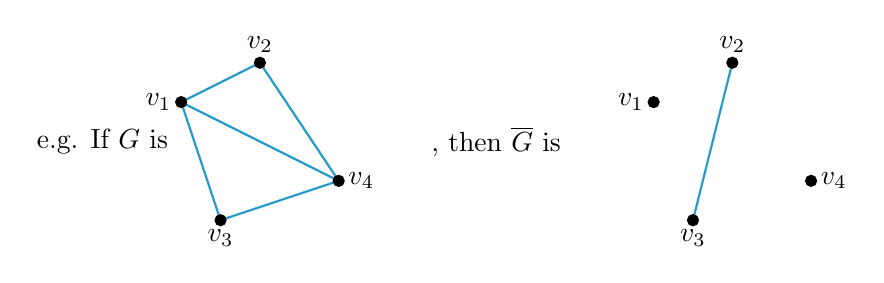
\begin{tikzpicture}[scale=1]
        \node at (-1, 0.5) {e.g. If $G$ is};
        
        % Graph G
        \begin{scope}[xshift=0cm]
            \coordinate (v1) at (0,1); \node[left] at (v1) {$v_1$};
            \coordinate (v2) at (1,1.5); \node[above] at (v2) {$v_2$};
            \coordinate (v3) at (0.5,-0.5); \node[below] at (v3) {$v_3$};
            \coordinate (v4) at (2,0); \node[right] at (v4) {$v_4$};
            
            \draw[cyan!80!black, thick] (v1)--(v2)--(v4)--(v3)--(v1)--(v4);
            
            \foreach \p in {v1,v2,v3,v4} \filldraw (\p) circle (2pt);
        \end{scope}
        
        \node at (4, 0.5) {, then $\overline{G}$ is};
        
        % Graph G_bar (Complement)
        \begin{scope}[xshift=6cm]
            \coordinate (u1) at (0,1); \node[left] at (u1) {$v_1$};
            \coordinate (u2) at (1,1.5); \node[above] at (u2) {$v_2$};
            \coordinate (u3) at (0.5,-0.5); \node[below] at (u3) {$v_3$};
            \coordinate (u4) at (2,0); \node[right] at (u4) {$v_4$};
            
            % Edges NOT in G: v2-v3 is the only missing edge in K4-e
            \draw[cyan!80!black, thick] (u2)--(u3);
            
            \foreach \p in {u1,u2,u3,u4} \filldraw (\p) circle (2pt);
        \end{scope}
    \end{tikzpicture}
    \end{center}
\end{enumerate}
\end{definition}

% 1.19 Definition
\begin{definition}
We call a graph $G$ \textbf{regular} if any of its vertices has the same degree. If this degree is $r$, we say that $G$ is \textbf{$r$-regular}.
\end{definition}

% 1.20 Remarks
\begin{remark}
\begin{enumerate}
    \item A graph $G$ is regular iff $\delta(G)=\Delta(G)$.
    \item $K_n$ is $(n-1)$-regular and $E_n$ is $0$-regular.
    \item An $r$-regular graph of order $n$ has $\frac{1}{2}nr$ many edges.
\end{enumerate}
\end{remark}

% 1.21 Example
\begin{example}
The graph below is 4-regular of order 6.
\begin{center}
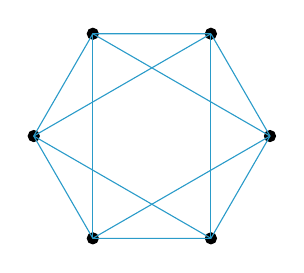
\begin{tikzpicture}
    % Octahedron graph projection
    \foreach \i in {1,...,6}
        \coordinate (v\i) at (60*\i:1.5);
    
    \foreach \i in {1,...,6} \filldraw (v\i) circle (2pt);
    
    \draw[cyan!80!black] (v1)--(v2)--(v3)--(v4)--(v5)--(v6)--(v1);
    \draw[cyan!80!black] (v1)--(v3); \draw[cyan!80!black] (v1)--(v5);
    \draw[cyan!80!black] (v2)--(v4); \draw[cyan!80!black] (v2)--(v6);
    \draw[cyan!80!black] (v3)--(v5); \draw[cyan!80!black] (v4)--(v6);
\end{tikzpicture}
\end{center}
\end{example}

\section{Subgraphs}

There are two ways in which one graph can be part of another graph.

% 1.22 Definition
\begin{definition}
\begin{enumerate}
    \item A graph $H$ is called a \textbf{subgraph} of some graph $G$, written $H \subseteq G$, if $V(H) \subseteq V(G)$ and $E(H) \subseteq E(G)$. We also say $G$ \textbf{contains} $H$.
    \item If $H \subseteq G$, we say that $H$ is an \textbf{induced subgraph} of $G$, written $H \sqsubseteq G$, if $E(H) = \{uv \in E(G) \mid u,v \in V(H)\}$.
\end{enumerate}
\end{definition}

% 1.23 Remark
\begin{remark}
\begin{enumerate}
    \item $H \subseteq G$ is induced if for any two vertices in $H$ we have: If they are adjacent in $G$, then they are adjacent in $H$.
    \item Every induced subgraph is a subgraph but not vice versa.
    \item If $G$ is a graph and $S \subseteq V(G)$, then there is only one induced subgraph $H \sqsubseteq G$ with vertex set $S$, i.e. $V(H)=S$. We denote this graph by $\langle S \rangle$ and call it the subgraph of $G$ induced by $S$.
\end{enumerate}
\end{remark}

% 1.24 Example
\begin{example}
Consider $G$ given as
\begin{center}
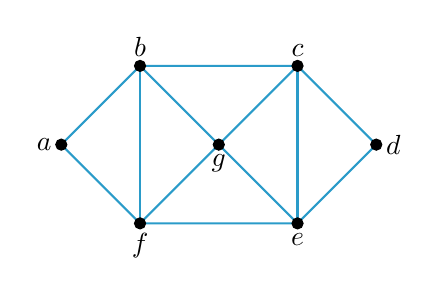
\begin{tikzpicture}[scale=1]
    % Main Graph G Coordinates
    \coordinate (g) at (0,0);
    \coordinate (b) at (-1,1); \coordinate (c) at (1,1);
    \coordinate (e) at (1,-1); \coordinate (f) at (-1,-1);
    \coordinate (a) at (-2,0); \coordinate (d) at (2,0);

    % Edges of G
    \draw[cyan!80!black, thick] (a)--(b)--(c)--(d)--(e)--(f)--(a);
    \draw[cyan!80!black, thick] (b)--(f); % Vertical
    \draw[cyan!80!black, thick] (c)--(e); % Vertical
    \draw[cyan!80!black, thick] (b)--(g)--(e); % Cross
    \draw[cyan!80!black, thick] (c)--(g)--(f); % Cross

    % Vertices
    \foreach \p/\pos/\label in {a/left/a, b/above/b, c/above/c, d/right/d, e/below/e, f/below/f, g/below/g}
        \filldraw (\p) circle (2pt) node[\pos] {$\label$};
\end{tikzpicture}
\end{center}

Then

\begin{center}
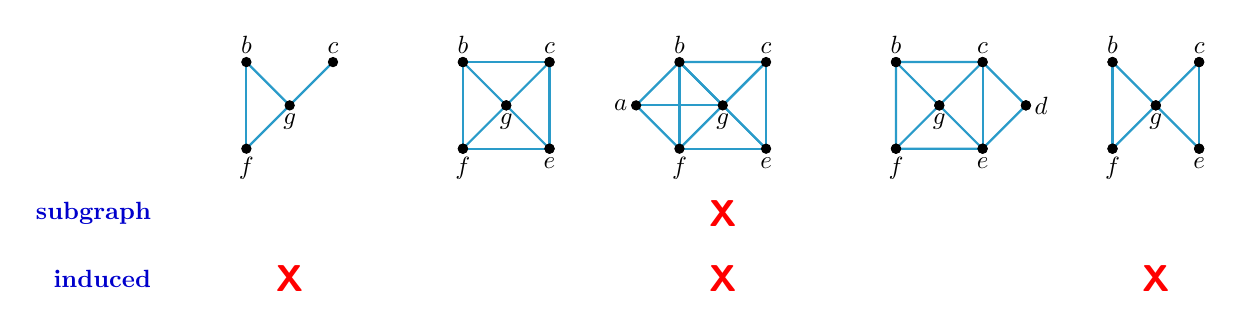
\begin{tikzpicture}[scale=0.55, every node/.style={scale=0.9}]
    % Define the standard node positions macro for consistency
    \def\nodes{
        \coordinate (g) at (0,0);
        \coordinate (b) at (-1,1); \coordinate (c) at (1,1);
        \coordinate (e) at (1,-1); \coordinate (f) at (-1,-1);
        \coordinate (a) at (-2,0); \coordinate (d) at (2,0);
    }

    % --- Row Labels ---
    \node[anchor=east, blue!80!black, font=\bfseries] at (-3, -2.5) {subgraph};
    \node[anchor=east, blue!80!black, font=\bfseries] at (-3, -4.0) {induced};

    % --- 1. Graph (b,c,f,g) ---
    \begin{scope}[xshift=0cm]
        \nodes
        \draw[cyan!80!black, thick] (b)--(f);
        \draw[cyan!80!black, thick] (b)--(g);
        \draw[cyan!80!black, thick] (g)--(c); 
        \draw[cyan!80!black, thick] (g)--(f); 
        \filldraw (b) circle (3pt) node[above] {$b$};
        \filldraw (c) circle (3pt) node[above] {$c$};
        \filldraw (f) circle (3pt) node[below] {$f$};
        \filldraw (g) circle (3pt) node[below] {$g$};
        
        % Marks
        \node[scale=1.5, green!60!black] at (0, -2.5) {\textbf{\checkmark}};
        \node[scale=1.5, red] at (0, -4.0) {\textbf{\sffamily X}};
    \end{scope}

    % --- 2. Graph (b,c,e,f,g - The Square with Cross) ---
    \begin{scope}[xshift=5cm]
        \nodes
        \draw[cyan!80!black, thick] (b)--(c)--(e)--(f)--(b); % Outer Box
        \draw[cyan!80!black, thick] (b)--(f); % Vertical
        \draw[cyan!80!black, thick] (c)--(e); % Vertical
        \draw[cyan!80!black, thick] (b)--(g)--(e); % Cross
        \draw[cyan!80!black, thick] (c)--(g)--(f); % Cross
        \foreach \p in {b,c,e,f,g} \filldraw (\p) circle (3pt);
        \filldraw (b) circle (3pt) node[above] {$b$};
        \filldraw (c) circle (3pt) node[above] {$c$};
        \filldraw (f) circle (3pt) node[below] {$f$};
        \filldraw (g) circle (3pt) node[below] {$g$};
        \filldraw (e) circle (3pt) node[below] {$e$};
        
        
        % Marks
        \node[scale=1.5, green!60!black] at (0, -2.5) {\textbf{\checkmark}};
        \node[scale=1.5, green!60!black] at (0, -4.0) {\textbf{\checkmark}};
    \end{scope}

    % --- 3. Graph (The Invalid one with a-g) ---
    \begin{scope}[xshift=10cm]
        \nodes
        \draw[cyan!80!black, thick] (a)--(b)--(c);
        \draw[cyan!80!black, thick] (b)--(f)--(e)--(c);
        \draw[cyan!80!black, thick] (b)--(g)--(c);
        \draw[cyan!80!black, thick] (b)--(g)--(e); % Cross
        \draw[cyan!80!black, thick] (c)--(g)--(f); % Cross
        \draw[cyan!80!black, thick] (b)--(g)--(e); % Cross
        \draw[cyan!80!black, thick] (c)--(g)--(f); % Cross
        \draw[cyan!80!black, thick] (a)--(f);
        \draw[cyan!80!black, thick] (a)--(g); % <--- The invalid edge
        \foreach \p/\pos/\label in {a/left/a, b/above/b, c/above/c, e/below/e, f/below/f, g/below/g}
        \filldraw (\p) circle (3pt) node[\pos] {$\label$};
        
        % Marks
        \node[scale=1.5, red] at (0, -2.5) {\textbf{\sffamily X}};
        \node[scale=1.5, red] at (0, -4.0) {\textbf{\sffamily X}};
    \end{scope}

    % --- 4. Graph (G without a) ---
    \begin{scope}[xshift=15cm]
        \nodes
        \draw[cyan!80!black, thick] (b)--(c)--(d)--(e)--(f)--(b);
        \draw[cyan!80!black, thick] (b)--(f);
        \draw[cyan!80!black, thick] (c)--(e);
        \draw[cyan!80!black, thick] (b)--(g)--(e);
        \draw[cyan!80!black, thick] (c)--(g)--(f);
        \foreach \p in {b,c,d,e,f,g} \filldraw (\p) circle (3pt);
        \foreach \p/\pos/\label in {b/above/b, c/above/c, d/right/d, e/below/e, f/below/f, g/below/g}
        \filldraw (\p) circle (3pt) node[\pos] {$\label$};
        
        % Marks
        \node[scale=1.5, green!60!black] at (0, -2.5) {\textbf{\checkmark}};
        \node[scale=1.5, green!60!black] at (0, -4.0) {\textbf{\checkmark}};
    \end{scope}

    % --- 5. Graph (The Bowtie) ---
    \begin{scope}[xshift=20cm]
        \nodes
        \draw[cyan!80!black, thick] (b)--(f);
        \draw[cyan!80!black, thick] (c)--(e);
        \draw[cyan!80!black, thick] (b)--(g)--(e);
        \draw[cyan!80!black, thick] (c)--(g)--(f);
        \foreach \p in {b,c,e,f,g} \filldraw (\p) circle (3pt);
        \foreach \p/\pos/\label in {b/above/b, c/above/c, e/below/e, f/below/f, g/below/g}
        \filldraw (\p) circle (3pt) node[\pos] {$\label$};
        
        % Marks
        \node[scale=1.5, green!60!black] at (0, -2.5) {\textbf{\checkmark}};
        \node[scale=1.5, red] at (0, -4.0) {\textbf{\sffamily X}};
    \end{scope}

\end{tikzpicture}
\end{center}
\end{example}

\section{Walks in Graphs}

% 1.25 Definition
\begin{definition}
A $(v_0, v_k)$-\textbf{walk} in a graph is a sequence of vertices $(v_0, v_1, \dots, v_k)$ s.t. any two consecutive vertices $v_i$ and $v_{i+1}$ are adjacent. We call the edges $\{v_0v_1, v_1v_2, \dots, v_{k-1}v_k\}$ the \textbf{edges of the walk}. We say that the walk is \textbf{closed} if $v_0=v_k$. The \textbf{length} of a walk is the number of edges in it (counting repetition).
\end{definition}

% 1.26 Definition
\begin{definition}
We distinguish the following types of walks:
\begin{itemize}
    \item A \textbf{trail} is a walk whose edges are pairwise distinct.
    \item A \textbf{circuit} is a closed walk whose edges are pairwise distinct.
    \item A \textbf{path} is a walk whose vertices are distinct.
    \item A \textbf{cycle} is a closed walk $(v_0, \dots, v_k=v_0)$ with $k \ge 3$ and whose vertices $v_0, \dots, v_{k-1}$ are pairwise distinct.
\end{itemize}
\end{definition}

% 1.27 Example
\begin{example}
Consider $G$ via
\begin{center}
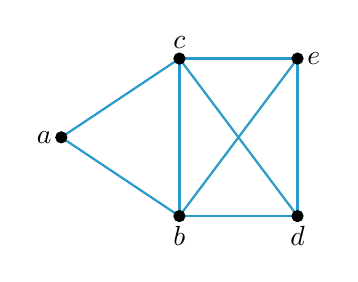
\begin{tikzpicture}[scale=1]
    % Coordinates based on drawing
    \coordinate (a) at (-2, 0);
    \coordinate (c) at (-0.5, 1);
    \coordinate (e) at (1, 1);
    \coordinate (b) at (-0.5, -1);
    \coordinate (d) at (1, -1);

    % Edges
    \draw[cyan!80!black, thick] (a) -- (c);
    \draw[cyan!80!black, thick] (a) -- (b);
    \draw[cyan!80!black, thick] (c) -- (b);
    \draw[cyan!80!black, thick] (c) -- (e);
    \draw[cyan!80!black, thick] (c) -- (d); % Cross
    \draw[cyan!80!black, thick] (b) -- (e); % Cross
    \draw[cyan!80!black, thick] (b) -- (d);
    \draw[cyan!80!black, thick] (e) -- (d);

    % Vertices
    \foreach \p/\pos/\label in {a/left/a, b/below/b, c/above/c, d/below/d, e/right/e}
        \filldraw (\p) circle (2pt) node[\pos] {$\label$};
\end{tikzpicture}
\end{center}

Give examples for a:

\begin{minipage}[t]{0.48\textwidth}
    \begin{itemize}
        \item \textbf{walk} $(d, b, c, d, b, a)$ \\
        $da$-walk, length 5
        \item \textbf{trail} $(d, c, a, b, c, e)$ \\
        $de$-trail, length 5
        \item \textbf{path} $(d, c, a, b, e)$ \\
        $de$-path, length 4
    \end{itemize}
\end{minipage}%
\begin{minipage}[t]{0.48\textwidth}
    \begin{itemize}
        \item \textbf{closed walk} $(e, b, c, a, b, d, e)$ \\
        $e$-closed walk, length 6
        \item \textbf{circuit} $(d, c, a, b, c, e, d)$ \\
        $d$-circuit, length 6
        \item \textbf{cycle} $(d, c, a, b, e, d)$ \\
        $d$-cycle, length 5
    \end{itemize}
\end{minipage}
\end{example}

% 1.28 Lemma
\begin{lemma}
If $\delta(G) \ge 2$, then $G$ contains a cycle as a subgraph.
\end{lemma}
\begin{proof}
Let $P = (v_0, \dots, v_k)$ be a path in $G$ of maximal length. This exists, as $G$ is finite. Further, as $\delta(G) \ge 2$, we get $k \ge 2$. As $\deg(v_0) \ge \delta(G) \ge 2$, $v_0$ has at least two neighbors. One of them is $v_1$. Let us denote the other one by $u$. If $u \ne v_i$ for all $1 \le i \le k$, then $\tilde{P} = (u, v_0, v_1, \dots, v_k)$ is still a path and of greater length than $P$, contradicting our assumptions. Hence, $u=v_i$ for some $1 \le i \le k$. But then the sequence $(v_0, v_1, \dots, v_i=u, v_0)$ is the desired cycle subgraph of $G$.
\end{proof}

% 1.29 Corollary
\begin{corollary}[Contrapositive]
If $G$ does not contain any cycles, then $\delta(G) \le 1$.
\end{corollary}

% 1.30 Theorem
\begin{theorem}
Every $uv$-walk in a graph contains a $uv$-path.
\end{theorem}
\begin{proof}
We proceed by strong induction on the length $n \ge 1$ of the walk.
\textbf{I.B. n=1.} If the $uv$-walk is of length one, then it is exactly $(u,v)$, which is also a path.
\textbf{I.S.} Assume every $uv$-walk of length at most $n \ge 1$ contains a $uv$-path (I.H.). Assume there is a $uv$-walk $W=(u=w_0, w_1, \dots, w_n, w_{n+1}=v)$ of length $n+1$. If $W$ is already a path, we are done. Otherwise there are $i,j$ s.t. $0 \le i < j \le n+1$ and $w_i = w_j$. But then the walk $\tilde{W}$ which arises from $W$ by deleting the vertices $w_{i+1}, \dots, w_{j-1}, w_j$, i.e. $\tilde{W} = (u=w_0, \dots, w_i, w_{j+1}, \dots, w_{n+1}=v)$ is still a $uv$-walk, but of length at most $n$. Using I.H., we know that $\tilde{W}$ contains a $uv$-path, whence also $W$ contains (the same) $uv$-path.
\end{proof}

\section{Connectivity}

% 1.31 Definition
\begin{definition}
A graph is \textbf{connected} if there exists an $uv$-path in $G$ for any vertices $u,v \in V(G)$. Otherwise, it is called \textbf{disconnected}.
\end{definition}

% Intuition (Unnumbered Header)
\par\vspace{0.5cm}\noindent
% This command forces the header to stay with the text
\needspace{4\baselineskip} 
{\large \underline{\textbf{Intuition}}}
\par\vspace{0.2cm}
A graph is connected if you could pick it up entirely by just lifting one vertex. If it is not connected, then the subgraph you lift that way is called a connected component.

% 1.32 Definition
\begin{definition}
A \textbf{connected component} of $G$ is a maximal connected induced subgraph of $G$. i.e. $C \sqsubseteq G$ is a connected component iff (i) $C$ is connected and (ii) for any $v \in V(G) \setminus V(C)$ the induced subgraph on $V(C) \cup \{v\}$ is \textbf{not} connected.
\end{definition}

% 1.33 Remark
\begin{remark}
$G$ is connected iff it has exactly one connected component.
\end{remark}

Even among connected graphs, there are different levels of being connected. E.g. the graph $K_5$

\begin{tikzpicture}[baseline=-0.5ex, scale=0.4]
    \foreach \i in {1,...,5} \coordinate (v\i) at (90+72*\i:0.5);
    \foreach \i in {1,...,5} \foreach \j in {\i,...,5} \draw[cyan!80!black] (v\i) -- (v\j);
    \foreach \i in {1,...,5} \filldraw (v\i) circle (2pt);
\end{tikzpicture}
``feels'' more connected than the graph

\begin{tikzpicture}[baseline=-0.5ex, scale=0.4]
    % Bowtie graph visualization
    \coordinate (c) at (0,0);
    \coordinate (l1) at (-0.6, 0.4);
    \coordinate (l2) at (-0.6, -0.4);
    \coordinate (r1) at (0.6, 0.4);
    \coordinate (r2) at (0.6, -0.4);
    
    \draw[cyan!80!black, thick] (l1)--(l2)--(c)--(l1); % Left triangle
    \draw[cyan!80!black, thick] (r1)--(r2)--(c)--(r1); % Right triangle
    
    \foreach \p in {c,l1,l2,r1,r2} \filldraw (\p) circle (2pt);
\end{tikzpicture}.
In order to properly describe this intuition, we need more notations.


% 1.34 Definition
\begin{definition}[Vertex and Edge Deletion]
Let $G$ be a graph, $S \subseteq V_G$ and $T \subseteq E_G$.
\begin{enumerate}
    \item By $G-S$ we denote the graph arising from $G$ by removing from $V_G$ all vertices in $S$ and their incident edges.
    \item If $S=\{v\}$, we write $G-v$.
    \item By $G-T$ we denote the graph arising from $G$ by removing only the edges in $T$, but no vertices.
    \item If $T=\{e\}$, we write $G-e$.
\end{enumerate}
\end{definition}

% 1.35 Example
\begin{example}
Consider $G$ as given below. Note that $G$ only has one connected component.
\begin{center}
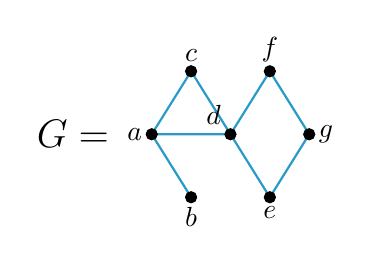
\begin{tikzpicture}[scale=1]
    % Coordinates for graph G
    \coordinate (a) at (0,0);
    \coordinate (b) at (0.5,-0.8);
    \coordinate (c) at (0.5,0.8);
    \coordinate (d) at (1,0);
    \coordinate (e) at (1.5,-0.8);
    \coordinate (f) at (1.5,0.8);
    \coordinate (g) at (2,0);

    % Main Label G=
    \node at (-1,0) {\Large $G=$};

    % Edges
    \draw[cyan!80!black, thick] (a)--(c)--(d)--(a)--(b);
    \draw[cyan!80!black, thick] (d)--(f)--(g)--(e)--(d);

    % Vertices
    \foreach \p/\pos/\label in {a/left/a, b/below/b, c/above/c, d/above left/d, e/below/e, f/above/f, g/right/g}
        \filldraw (\p) circle (2pt) node[\pos] {$\label$};
\end{tikzpicture}
\end{center}

Then $G-d$ is
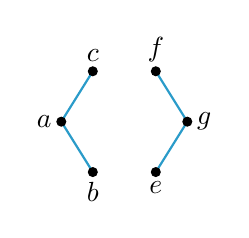
\begin{tikzpicture}[scale=0.8, baseline=-0.5ex]
    \coordinate (a) at (0,0);
    \coordinate (b) at (0.5,-0.8);
    \coordinate (c) at (0.5,0.8);
    % d is removed
    \coordinate (e) at (1.5,-0.8);
    \coordinate (f) at (1.5,0.8);
    \coordinate (g) at (2,0);

    \draw[cyan!80!black, thick] (a)--(c); \draw[cyan!80!black, thick] (a)--(b);
    \draw[cyan!80!black, thick] (f)--(g)--(e);

    \foreach \p/\pos/\label in {a/left/a, b/below/b, c/above/c, e/below/e, f/above/f, g/right/g}
        \filldraw (\p) circle (2pt) node[\pos] {$\label$};
\end{tikzpicture}
and has 2 connected components. \\
The vertex $d$ is called a \textbf{\color{red}cut vertex}.

Further, $G-\{e,f\}$ is
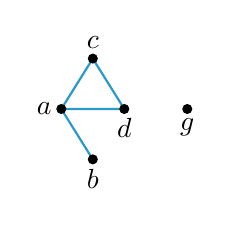
\begin{tikzpicture}[scale=0.8, baseline=-0.5ex]
    \coordinate (a) at (0,0);
    \coordinate (b) at (0.5,-0.8);
    \coordinate (c) at (0.5,0.8);
    \coordinate (d) at (1,0);
    \coordinate (g) at (2,0);

    \draw[cyan!80!black, thick] (a)--(c)--(d)--(a)--(b);
    % e, f removed so their edges are gone. g is isolated.

    \foreach \p/\pos/\label in {a/left/a, b/below/b, c/above/c, d/below/d, g/below/g}
        \filldraw (\p) circle (2pt) node[\pos] {$\label$};
\end{tikzpicture}
. It also has 2 connected components. \\
The set $\{e,f\}$ is called a \textbf{\color{red}cut set}.

Further, $G-ab$ is
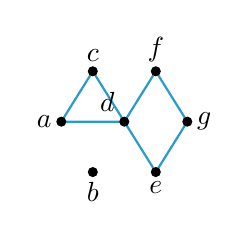
\begin{tikzpicture}[scale=0.8, baseline=-0.5ex]
    \coordinate (a) at (0,0);
    \coordinate (b) at (0.5,-0.8);
    \coordinate (c) at (0.5,0.8);
    \coordinate (d) at (1,0);
    \coordinate (e) at (1.5,-0.8);
    \coordinate (f) at (1.5,0.8);
    \coordinate (g) at (2,0);

    % Remove ab edge (a--b)
    \draw[cyan!80!black, thick] (a)--(c)--(d)--(a); % Triangle a-c-d
    \draw[cyan!80!black, thick] (d)--(f)--(g)--(e)--(d);

    \foreach \p/\pos/\label in {a/left/a, b/below/b, c/above/c, d/above left/d, e/below/e, f/above/f, g/right/g}
        \filldraw (\p) circle (2pt) node[\pos] {$\label$};
\end{tikzpicture}
Again, it has 2 connected components. \\
We call the edge $ab$ a \textbf{\color{red}bridge}.
\end{example}

% 1.36 Definition
\begin{definition}
Let $G$ be a graph.
\begin{enumerate}
    \item We call $v \in V_G$ a \textbf{cut vertex} if $G-v$ has more connected components than $G$ itself.
    \item We call $e \in E_G$ a \textbf{bridge} if $G-e$ has more connected components than $G$ itself.
    \item We call $S \subseteq V_G$ a \textbf{cut set} if $G-S$ is disconnected.
    \item A connected graph which does not contain any cut vertices is called \textbf{non-separable}.
\end{enumerate}
\end{definition}

% 1.37 Observation
\topic{Observation}
\begin{enumerate}
    \item If $G$ is connected then $v$ is a cut vertex of $G$ iff $\{v\}$ is a cut set.
    \item The vertex $v$ is a cut vertex iff there are vertices $u$ and $w$, different from $v$ s.t. every $uw$-path uses $v$.
    \item A graph has no cut sets iff it is a complete graph.
\end{enumerate}

% 1.38 Definition
\begin{definition}
For a non-complete graph $G$, we define its \textbf{connectivity} $\kappa(G)$ as the minimal size of a cut set. For $K_n$, we set $\kappa(K_n) = n-1$.
\end{definition}


% 1.39 Lemma
\begin{lemma}
If $G$ is a nonseparable graph of order at least 3, then $\delta(G) \ge 2$ and every vertex of $G$ is contained in a cycle.
\end{lemma}

\begin{proof}
Consider $G$ nonseparable with $|G| \ge 3$. By definition, $G$ is connected, i.e. $\delta(G) \ge 1$.

First we show that $\delta(G) \ge 2$. Otherwise, we have $\delta(G)=1$, i.e. there is some vertex $v$ s.t. $\deg(v)=1$. Let $u$ be the unique neighbor of $v$ and $w$ any other vertex of $G$ (which exists as $|G| \ge 3$). Then clearly any $vw$-path must use the unique neighbor $u$ of $v$, whence $u$ is a cut vertex. This contradicts the fact that $G$ is inseparable. Hence, $\delta(G) \ge 2$, as desired.

\begin{center}
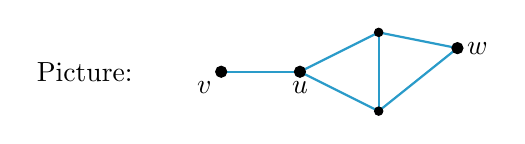
\begin{tikzpicture}[scale=1]
    \node[left] at (-1,0) {Picture:};
    
    \coordinate (v) at (0,0);
    \coordinate (u) at (1,0);
    \coordinate (x1) at (2,0.5);
    \coordinate (x2) at (2,-0.5);
    \coordinate (w) at (3,0.3);
    
    \draw[cyan!80!black, thick] (v) -- (u);
    \draw[cyan!80!black, thick] (u) -- (x1) -- (w);
    \draw[cyan!80!black, thick] (u) -- (x2) -- (w);
    \draw[cyan!80!black, thick] (x1) -- (x2);
    
    \filldraw (v) circle (2pt) node[below left] {$v$};
    \filldraw (u) circle (2pt) node[below] {$u$};
    \filldraw (w) circle (2pt) node[right] {$w$};
    \filldraw (x1) circle (1.5pt);
    \filldraw (x2) circle (1.5pt);
\end{tikzpicture}
\end{center}

\vspace{0.3cm}

Now, consider $v \in V_G$ arbitrary. We want to show that $v$ is contained in a cycle in $G$. As $\delta(G) \ge 2$, $v$ has at least 2 neighbors, say $u$ and $w$. 
As $G$ is nonseparable, $G-v$ is still connected. In particular, there is a $uw$-path $(u=x_0, x_1, x_2, \dots, x_k=w)$ in $G-v$. But then the walk $(x_0=u, x_1, \dots, x_k=w, v, x_0=u)$ is the desired cycle containing $v$.

\begin{center}
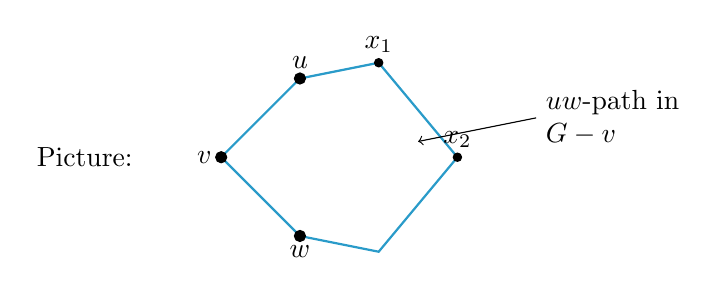
\begin{tikzpicture}[scale=1]
    \node[left] at (-1,0) {Picture:};
    
    \coordinate (v) at (0,0);
    \coordinate (u) at (1,1);
    \coordinate (w) at (1,-1);
    
    % Draw v connected to neighbors
    \draw[cyan!80!black, thick] (v) -- (u);
    \draw[cyan!80!black, thick] (v) -- (w);
    
    % Draw the path in G-v
    \coordinate (x1) at (2, 1.2);
    \coordinate (x2) at (3, 0);
    \coordinate (x3) at (2, -1.2);
    
    \draw[cyan!80!black, thick] (u) -- (x1) -- (x2) -- (x3) -- (w);
    
    % Nodes
    \filldraw (v) circle (2pt) node[left] {$v$};
    \filldraw (u) circle (2pt) node[above] {$u$};
    \filldraw (w) circle (2pt) node[below] {$w$};
    
    \filldraw (x1) circle (1.5pt) node[above] {$x_1$};
    \filldraw (x2) circle (1.5pt) node[above] {$x_2$};
    
    % Annotation
    \draw[->, thin, black] (4, 0.5) -- (2.5, 0.2) node[right, at start, align=left] {$uw$-path in \\ $G-v$};
\end{tikzpicture}
\end{center}
\end{proof}

% 1.40 Definition
\begin{definition}
We say that $G$ is \textbf{\color{red}$k$-connected} if $\kappa(G) \ge k$, i.e. if $G$ is connected and $G-S$ is still connected for any $S \subseteq V_G$ with $|S| < k$.
\end{definition}

% 1.41 Lemma
\begin{lemma}
The following hold:
\begin{enumerate}
    \item[1)] $G$ is connected iff $\kappa(G) \ge 1$.
    \item[2)] $G$ is 1-connected iff $G$ is connected.
    \item[3)] $G$ is 2-connected iff $G$ is connected and has no cut vertices.
    \item[4)] $G$ is 2-connected iff $G$ is non-separable.
    \item[5)] If $G$ is 2-connected, then it contains at least one cycle (for $|G| \ge 3$).
    \item[6)] If $G$ is $k$-connected, then $G$ is $j$-connected for all $j \le k$.
    \item[7)] $|G| > \kappa(G)$.
    \item[8)] $\kappa(G) \le \delta(G)$.
\end{enumerate}
\end{lemma}

\begin{proof}
1)--6) are easy observations -- verify them by yourselves.

\vspace{0.3cm}
\noindent \underline{7)} If $G=K_n$, then $|G|=n > n-1 = \kappa(G)$. Otherwise, assume $\kappa(G)=k$, i.e. ex. $S \subseteq V_G$ s.t. $|S|=k$ and $G-S$ is disconnected. For $G-S$ to be disconnected, it must contain at least 2 vertices, whence
\[ |G| \ge |S|+2 = \kappa(G)+2 > \kappa(G). \]

\vspace{0.3cm}
\noindent \underline{8)} Assume $\kappa(G) > \delta(G)$ and let $v \in V_G$ s.t. $\deg(v) = \delta(G)$. Note that $|G| > \kappa(G) > \delta(G) = |N(v)|$, whence $G-N(v)$ contains at least one vertex besides $v$. But clearly, $G-N(v)$ is disconnected (as $\deg^{G-N(v)}(v)=0$).
Hence, $N(v)$ is a cut set and $\kappa(G) \le |N(v)| = \delta(G)$, contradicting the assumptions.
\end{proof}

\section{Bipartite Graphs}

% 1.42 Definition
\begin{definition}
A graph $G$ is called \textbf{bipartite} if we can partition the vertex set $V_G$ into two disjoint sets $V_G = X \cup Y$ s.t. every edge of $G$ has one end vertex in $X$ and the other in $Y$.
\end{definition}

% 1.43 Example
\begin{example}
Consider $G:=$
\begin{center}
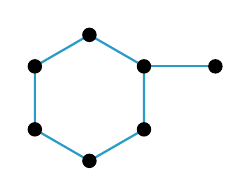
\begin{tikzpicture}[scale=0.8]
    % Coordinates for the initial cycle layout
    \foreach \i in {1,...,6}
        \coordinate (v\i) at (90 + 60 - 60*\i : 1);
    \coordinate (v7) at (2, 0.5); % The tail node

    % Edges
    \draw[cyan!80!black, thick] (v1)--(v2)--(v3)--(v4)--(v5)--(v6)--(v1);
    \draw[cyan!80!black, thick] (v2)--(v7);

    % Vertices
    \foreach \p in {v1,v2,v3,v4,v5,v6,v7} \filldraw (\p) circle (3pt);
\end{tikzpicture}
\end{center}

We can partition the vertices of $G$ into two sets via
$X = \{x_1, x_2, x_3\}$ and $Y = \{y_1, y_2, y_3, y_4\}$.

\begin{center}
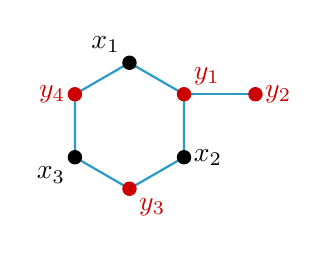
\begin{tikzpicture}[scale=0.8]
    % Same layout, but colored nodes
    \foreach \i in {1,...,6}
        \coordinate (n\i) at (90 + 60 - 60*\i : 1);
    \coordinate (n7) at (2, 0.5);

    % Edges
    \draw[cyan!80!black, thick] (n1)--(n2)--(n3)--(n4)--(n5)--(n6)--(n1);
    \draw[cyan!80!black, thick] (n2)--(n7);

    % Colored Vertices based on partition logic (Alternating)
    % Let's map visual to labels:
    % Top left (n1) = Black (x1)
    % Top right (n2) = Red (y1)
    % Right tail (n7) = Red (y2) ?? Wait, if n2 is red, n7 must be black?
    % Let's follow the bipartite logic: Neighbors must have diff colors.
    
    % Notes show:
    % Cycle 6: Black, Red, Black, Red, Black, Red.
    % Tail connected to a Red node must be Black? Or vice versa.
    
    % Let's follow the notes specific coloring visual:
    % Top-Left: Black (x1)
    % Top-Right: Red (y1)
    % Right: Black (x2)
    % Bottom-Right: Red (y3)
    % Bottom-Left: Black (x3)
    % Left: Red (y4)
    % Tail node connected to x2 (Black) -> Red (y2)
    
    \filldraw (n1) circle (3pt) node[above left] {$x_1$}; % Black
    \filldraw[red!80!black] (n2) circle (3pt) node[above right] {$y_1$}; % Red
    \filldraw (n3) circle (3pt) node[right] {$x_2$}; % Black
    \filldraw[red!80!black] (n7) circle (3pt) node[right] {$y_2$}; % Red (Tail)
    
    \filldraw[red!80!black] (n4) circle (3pt) node[below right] {$y_3$}; % Red
    \filldraw (n5) circle (3pt) node[below left] {$x_3$}; % Black
    \filldraw[red!80!black] (n6) circle (3pt) node[left] {$y_4$}; % Red
    
\end{tikzpicture}
\end{center}

Rearranging the position of the vertices makes it clear that $G$ is bipartite:

\begin{center}
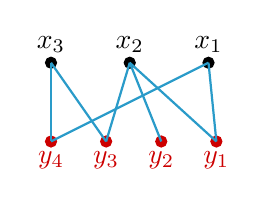
\begin{tikzpicture}[scale=1]
    % Top Row (X - Black)
    \coordinate (x3) at (0, 1);
    \coordinate (x2) at (1, 1);
    \coordinate (x1) at (2, 1);
    
    % Bottom Row (Y - Red)
    \coordinate (y4) at (0, 0);
    \coordinate (y3) at (0.7, 0);
    \coordinate (y2) at (1.4, 0);
    \coordinate (y1) at (2.1, 0);
    
    % Labels
    \filldraw (x3) circle (2pt) node[above] {$x_3$};
    \filldraw (x2) circle (2pt) node[above] {$x_2$};
    \filldraw (x1) circle (2pt) node[above] {$x_1$};
    
    \filldraw[red!80!black] (y4) circle (2pt) node[below] {$y_4$};
    \filldraw[red!80!black] (y3) circle (2pt) node[below] {$y_3$};
    \filldraw[red!80!black] (y2) circle (2pt) node[below] {$y_2$};
    \filldraw[red!80!black] (y1) circle (2pt) node[below] {$y_1$};
    
    % Edges based on the cycle structure
    % x1-y1, y1-x2, x2-y2(tail), x2-y3, y3-x3, x3-y4, y4-x1
    \draw[cyan!80!black, thick] (x1)--(y1);
    \draw[cyan!80!black, thick] (y1)--(x2);
    \draw[cyan!80!black, thick] (x2)--(y2);
    \draw[cyan!80!black, thick] (x2)--(y3);
    \draw[cyan!80!black, thick] (y3)--(x3);
    \draw[cyan!80!black, thick] (x3)--(y4);
    \draw[cyan!80!black, thick] (y4)--(x1);
    
\end{tikzpicture}
\end{center}
We see that there are no edges between any two vertices in $X$ or in $Y$.
\end{example}

% 1.44 Remark
\begin{remark}
A graph $G$ is bipartite if and only if we can color the vertices of $G$ with two colors s.t. the end vertices of each edge have different colors.
\end{remark}

% 1.45 Definition
\begin{definition}
Let $m,n \in \mathbb{Z}_+$. The \textbf{complete bipartite graph} $K_{m,n}$ is the bipartite graph with $X=\{x_1, \dots, x_m\}$, $Y=\{y_1, \dots, y_n\}$, $V_G=X \cup Y$ and $E_G = \{xy \mid x \in X, y \in Y\}$.
\end{definition}

% 1.46 Example
\begin{example}
Below are some examples of complete bipartite graphs.
\begin{center}
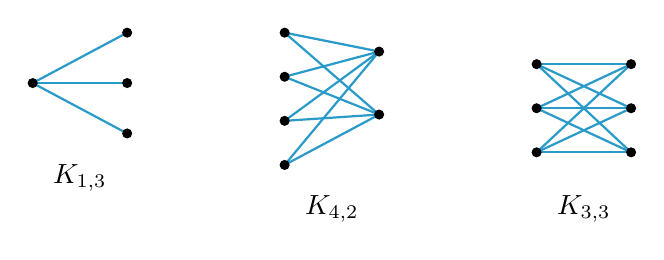
\begin{tikzpicture}[scale=0.8]
    % K_1,3
    \begin{scope}[xshift=0cm]
        \coordinate (x1) at (0, 0); % Left node
        \coordinate (y1) at (1.5, 0.8);
        \coordinate (y2) at (1.5, 0);
        \coordinate (y3) at (1.5, -0.8);
        
        \foreach \y in {y1,y2,y3} \draw[cyan!80!black, thick] (x1) -- (\y);
        
        \filldraw (x1) circle (2pt);
        \foreach \y in {y1,y2,y3} \filldraw (\y) circle (2pt);
        
        \node at (0.75, -1.5) {$K_{1,3}$};
    \end{scope}

    % K_4,2
    \begin{scope}[xshift=4cm]
        % Left column (4 nodes)
        \foreach \i in {1,...,4} \coordinate (l\i) at (0, 1.5 - 0.7*\i);
        % Right column (2 nodes)
        \coordinate (r1) at (1.5, 0.5);
        \coordinate (r2) at (1.5, -0.5);
        
        \foreach \i in {1,...,4} {
            \draw[cyan!80!black, thick] (l\i) -- (r1);
            \draw[cyan!80!black, thick] (l\i) -- (r2);
            \filldraw (l\i) circle (2pt);
        }
        \filldraw (r1) circle (2pt); \filldraw (r2) circle (2pt);
        
        \node at (0.75, -2) {$K_{4,2}$};
    \end{scope}

    % K_3,3
    \begin{scope}[xshift=8cm]
        % Left column (3 nodes)
        \foreach \i in {1,...,3} \coordinate (l\i) at (0, 1 - 0.7*\i);
        % Right column (3 nodes)
        \foreach \i in {1,...,3} \coordinate (r\i) at (1.5, 1 - 0.7*\i);
        
        \foreach \i in {1,...,3} \foreach \j in {1,...,3}
            \draw[cyan!80!black, thick] (l\i) -- (r\j);
            
        \foreach \i in {1,...,3} {
            \filldraw (l\i) circle (2pt);
            \filldraw (r\i) circle (2pt);
        }
        
        \node at (0.75, -2) {$K_{3,3}$};
    \end{scope}
\end{tikzpicture}
\end{center}
\end{example}
The following theorem helps us decide whether or not a given graph is bipartite.


% 1.47 Theorem
\begin{theorem}
A graph is bipartite iff it does not contain odd cycles.
\end{theorem}

\begin{proof}
``$\Rightarrow$'': Assume $G$ is bipartite and nevertheless there is a cycle of odd length, say $(x_0, x_1, \dots, x_{2k}, x_{2k+1}=x_0)$. By Remark 1.44, we can color $V_G$ in two colors, $C1$ and $C2$, s.t. adjacent vertices have different colors. Then, if $x_0$ has color $C1$, $x_1$ has color $C2$ whence $x_2$ has color $C1$. That way we see that the color of $x_i$ is 
\[ \begin{cases} C1 \text{ if } i \text{ is even} \\ C2 \text{ if } i \text{ is odd} \end{cases}. \]
Following that logic, the vertex $x_0 = x_{2k+1}$ should have color $C1$ and color $C2$ at the same time, which is a contradiction.

``$\Leftarrow$'': Now consider that $G$ does not contain odd cycles. We will show that $G$ is bipartite by providing a partition. We may assume that $G$ is connected as otherwise we work component per component.
Pick $v \in V_G$ arbitrary and define
\[ X = \{w \in V_G \mid \text{the shortest } vw \text{ path has even length}\} \text{ and} \]
\[ Y = \{w \in V_G \mid \text{the shortest } vw \text{ path has odd length}\}. \]
Clearly, $X$ and $Y$ are disjoint. We will show that there are no adjacent vertices in $X$ or $Y$ respectively. Note that $v \in X$.

Aiming for a contradiction, assume that there are vertices $w_1, w_2 \in X$ which are adjacent. Clearly, $w_1 \ne v$, as otherwise the shortest $vw_2$-path was exactly $vw_2$ of length 1. Similarly, $w_2 \ne v$. Let $P_1 = (v=x_0, x_1, \dots, x_{2k}=w_1)$ and $P_2 = (v=y_0, y_1, \dots, y_{2\ell}=w_2)$ be the shortest $vw_1$- and $vw_2$-paths.
Suppose that $x_i = y_j$ for some $0 < i \le 2k$ and $0 < j \le 2\ell$.
If $i < j$, then $(v=x_0, x_1, \dots, x_i, y_{j+1}, \dots, y_{2\ell}=w_2)$ is a $vw_2$ path shorter than $P_2$, a contradiction. Similarly, $j < i$ is impossible, whence $i=j$, whenever $x_i=y_j$.

Now, pick the largest $i$ s.t. $x_i=y_i$. As $x_0=v=y_0$, such an $i$ always exists. Then we obtain the following cycle
\[ C = (\underbrace{x_i, x_{i+1}, \dots, x_{2k}}_{2k-i}=w_1, \underbrace{w_2}_{1}=y_{2\ell}, \underbrace{y_{2\ell-1}, \dots, y_{i+1}}_{2\ell-i}, y_i=x_i). \]
This is a cycle, as $P_1$ and $P_2$ were paths and $i$ was maximal s.t. $x_i=y_i$. Further, the length of $C$ is odd, as it equals
\[ (2k-i) + 1 + (2\ell-i) = 2(k+\ell-i) + 1. \]
This contradicts our assumption that $G$ does not contain odd cycles. We hence proved that no two vertices $w_1$ and $w_2$ from $X$ can be adjacent.
The arguments for $v_1, v_2 \in Y$ is analogous (try to write it down).
This concludes the proof.
\end{proof}

\section{Graph Isomorphisms}

In Example 1.43, we rearranged the given graph $G_1$ as $G_2$.
\begin{center}
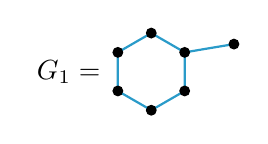
\begin{tikzpicture}[scale=0.7, baseline=(current bounding box.center)]
    % G1: Cycle with tail
    \foreach \i in {1,...,6} \coordinate (v\i) at (90+60-60*\i:0.7);
    \coordinate (v7) at (1.5, 0.5);
    \draw[cyan!80!black, thick] (v1)--(v2)--(v3)--(v4)--(v5)--(v6)--(v1);
    \draw[cyan!80!black, thick] (v2)--(v7);
    \foreach \p in {v1,v2,v3,v4,v5,v6,v7} \filldraw (\p) circle (2.5pt);
    \node at (-1.5,0) {$G_1=$};
\end{tikzpicture}
\hspace{1cm} as \hspace{1cm}
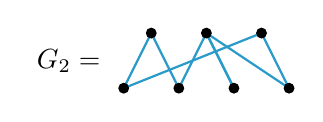
\begin{tikzpicture}[scale=0.7, baseline=(current bounding box.center)]
    % G2: Bipartite layout
    % Top row
    \foreach \i in {1,2,3} \coordinate (t\i) at (\i-1, 0.5);
    % Bottom row
    \foreach \i in {1,2,3,4} \coordinate (b\i) at (\i-1.5, -0.5);
    
    % Edges (Schematic bipartite connections)
    \draw[cyan!80!black, thick] (t1)--(b1); \draw[cyan!80!black, thick] (t1)--(b2);
    \draw[cyan!80!black, thick] (t2)--(b2); \draw[cyan!80!black, thick] (t2)--(b3);
    \draw[cyan!80!black, thick] (t2)--(b3); \draw[cyan!80!black, thick] (t3)--(b4);
    \draw[cyan!80!black, thick] (t2)--(b4); \draw[cyan!80!black, thick] (t3)--(b1);
    
    \foreach \p in {t1,t2,t3,b1,b2,b3,b4} \filldraw (\p) circle (2.5pt);
    \node at (-1.5,0) {$G_2=$};
\end{tikzpicture}
\end{center}

We understand $G_1$ and $G_2$ as the same, even though on the first glance, they look very similar. Another example is given by
\begin{center}
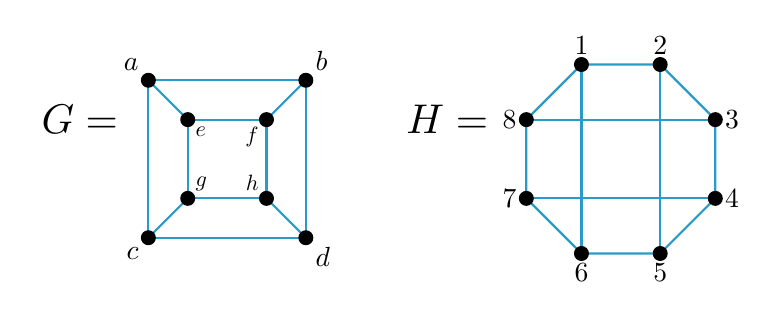
\begin{tikzpicture}[scale=1]
    % --- Graph G: Cube Projection (Square in Square) ---
    \begin{scope}[xshift=0cm]
        \node[left, scale=1.5] at (-1.2, 0.5) {$G=$};
        
        % Outer Square
        \coordinate (a) at (-1,1); \node[above left] at (a) {$a$};
        \coordinate (b) at (1,1);  \node[above right] at (b) {$b$};
        \coordinate (d) at (1,-1); \node[below right] at (d) {$d$};
        \coordinate (c) at (-1,-1); \node[below left] at (c) {$c$};
        
        % Inner Square
        \coordinate (e) at (-0.5,0.5); \node[below right, scale=0.8] at (e) {$e$};
        \coordinate (f) at (0.5,0.5);  \node[below left, scale=0.8] at (f) {$f$};
        \coordinate (h) at (0.5,-0.5); \node[above left, scale=0.8] at (h) {$h$};
        \coordinate (g) at (-0.5,-0.5); \node[above right, scale=0.8] at (g) {$g$};
        
        % Edges
        \draw[cyan!80!black, thick] (a)--(b)--(d)--(c)--(a); % Outer
        \draw[cyan!80!black, thick] (e)--(f)--(h)--(g)--(e); % Inner
        \draw[cyan!80!black, thick] (a)--(e);
        \draw[cyan!80!black, thick] (b)--(f);
        \draw[cyan!80!black, thick] (d)--(h);
        \draw[cyan!80!black, thick] (c)--(g);
        
        \foreach \p in {a,b,c,d,e,f,g,h} \filldraw (\p) circle (2.5pt);
    \end{scope}

    

    % --- Graph H: Circular Ladder (Octagon with cross links) ---
    \begin{scope}[xshift=5cm]
        \node[left, scale=1.5] at (-1.5, 0.5) {$H=$};
        
        % 8 points on a circle (rotated so 1 is top, 2 is top-right etc)
        % Notes show 1 top-left, 2 top-right. Let's align to a square-like octagon.
        \coordinate (n1) at (-0.5, 1.2); \node[above] at (n1) {1};
        \coordinate (n2) at (0.5, 1.2);  \node[above] at (n2) {2};
        \coordinate (n3) at (1.2, 0.5);  \node[right] at (n3) {3};
        \coordinate (n4) at (1.2, -0.5); \node[right] at (n4) {4};
        \coordinate (n5) at (0.5, -1.2); \node[below] at (n5) {5};
        \coordinate (n6) at (-0.5, -1.2); \node[below] at (n6) {6};
        \coordinate (n7) at (-1.2, -0.5); \node[left] at (n7) {7};
        \coordinate (n8) at (-1.2, 0.5);  \node[left] at (n8) {8};

        % Outer Cycle
        \draw[cyan!80!black, thick] (n1)--(n2)--(n3)--(n4)--(n5)--(n6)--(n7)--(n8)--(n1);
        
        % Cross connections (1-5, 2-6, 3-7, 4-8 based on isomorphism)
        % Actually, in the notes drawing it looks like horizontal/vertical bars.
        % 8-3, 7-4, 1-6, 2-5? No, let's look at the isomorphism text.
        % a->1, b->2, c->8, d->3.
        % a-b is an edge -> 1-2 is an edge. (Yes)
        % a-c is an edge -> 1-8 is an edge. (Yes)
        % c-d is an edge -> 8-3 is an edge? No, c-d in G connects (-1,-1) to (1,-1).
        
        % Let's just reproduce the VISUAL of H from the notes without overthinking the math isomorphism verification.
        % Visual H: Octagon shape.
        % Horizontal bars: 8-3, 7-4.
        % Vertical bars: 1-6, 2-5?
        % Let's look at the "H=" drawing in the handwritten note.
        % It looks like an octagon with 1,2 top, 3,4 right, 5,6 bottom, 7,8 left.
        % And it has cross bars: 1-6, 2-5, 8-3, 7-4.
        
        \draw[cyan!80!black, thick] (n1)--(n6);
        \draw[cyan!80!black, thick] (n2)--(n5);
        \draw[cyan!80!black, thick] (n8)--(n3);
        \draw[cyan!80!black, thick] (n7)--(n4);

        \foreach \p in {n1,n2,n3,n4,n5,n6,n7,n8} \filldraw (\p) circle (2.5pt);
    \end{scope}
\end{tikzpicture}
\end{center}

We can relabel the vertices of $G$ via $a \mapsto 1, b \mapsto 2, c \mapsto 8, d \mapsto 3, e \mapsto 7, f \mapsto 4, g \mapsto 6$ and $h \mapsto 5$ and obtain $H$. The aim of this section is to formalise this concept.

% 1.48 Definition
\begin{definition}
We say that a graph $G$ is \textbf{\color{red}isomorphic} to a graph $H$ if there exists a bijection $\varphi: V_G \to V_H$ s.t. for any $u,v \in V_G$ we have that $\{u,v\} \in E_G$ if and only if $\{\varphi(u), \varphi(v)\} \in E_H$. Then, the map $\varphi$ is called an \textbf{\color{red}isomorphism} and we write \textbf{\color{red}$G \cong H$}.
\end{definition}

% 1.49 Remark
\begin{remark}
Let $G \cong H$ via $\varphi: V_G \to V_H$. Then:
\begin{enumerate}
    \item[1)] $|V_G|=|V_H|$ and $|E_G|=|E_H|$ and $\overline{G} \cong \overline{H}$.
    \item[2)] The degree sequence of $G$ equals the degree sequence of $H$.
    \item[3)] $G$ is connected iff $H$ is connected.
    \item[4)] $\deg_G(v) = \deg_H(\varphi(v))$ for all $v \in V_G$.
\end{enumerate}
\end{remark}